% Lezione 3.1
\documentclass[../template]{subfiles}

\begin{document}
\section{Architetture Avanzate}
\subsection{Prestazione dei calcolatori}
Con benchmark si definisce un set di programmi differenti che rappresentano a grandi linee task frequenti eseguiti dal calcolatore.
Per confrontare le prestazioni di diversi calcolatori, viene eseguito lo stesso benchmark e si paragonano i diversi tempi di esecuzione.

\def\tcpu{T_\text{cpu}}

\subsection{Prestazione della CPU}
Sull'intero tempo di esecuzione di un programma, $\tcpu$ (\textit{Tempo di CPU}) è definito come l'effettivo tempo in cui la CPU è impiegata nell'esecuzione del task: $\tcpu = N_{cc} T_{ck}$, dove $N_{cc}$ è il numero di cicli di clock.
\\
Il metodo più semplice per calcolarlo è attraverso il CPI (\textit{Clock Per Instruction}) , ovvero il numero di cicli di clock mediamente richiesti da un istruzione: $\mathit{CPI} = N_{cc}/N$ dove $N$ è il numero di istruzioni in un programma.

Per calcolare il CPI medio, occorre conoscere il CPI di ogni istruzione, e la frequenza con la quale l'istruzione
$i$-esima viene eseguita $F_i$.
\[
    \mathit{CPI} = \sum_i F_i \times \mathit{CPI}_i = \sum_i \frac{N_i}{N} \mathit{CPI}_i
\]
Da cui:
\[
    \tcpu = N \times \mathit{CPI} \times T_{ck}
\]
Le architetture RISC, si concentrano nel ridurre il più possibile $\mathit{CPI}_i$, riducendo il numero di cicli di clock richiesti da ogni istruzione.
Il numero ridotto di istruzioni dell'architettura, si risente nella scrittura dei programmi, dove, per svolgere lo stesso compito, più istruzioni sono richieste, aumentando il CPI.

MIPS (\textit{Mega Instruction Per Second}) e MFLOPS (\textit{Mega FLoating Point Operation Per Second}) definite come
$\mathit{MIPS} = N / (\mathit{CPU}_\mathit{time} * 10^6) = f_\mathit{ck} / \mathit{CPI}$ sono utilizzate come unità per misurare le prestazioni.
Dipendono entrambe dal $\mathit{CPI}$ medio e quindi dal benchmark.

Il numero di MIPS non dipende da $N$, pertanto a parità MIPS e benchmark otteniamo valori diversi di
$\mathit{CPU}_\mathit{time}$ se $N$ cambia.
Ne consegue che due CPU sono paragonabili con lo stesso benchmark solamente se hanno lo stesso set di istruzioni.

\subsection{Architetture Pipeline}
Questa architettura è la soluzione più efficace per aumentare la velocità di una CPU, aumentando il numero di istruzioni eseguite nell'unità di tempo (throughput).
Diversamente dall'architettura multiciclo, tiene le istruzioni separate in più cicli di clock, rendendone possibile la loro esecuzione in parallelo.
\\
I segnali sono trasmessi di fase in fase attraverso registri di latch.

In generale, chiamato $\tau$ il tempo di clock, supponendo la divisione in $k$ stadi, $n$ istruzioni vengono elaborate in $T_k = (k + (n-1)) \cdot \tau$.
\\
L'aumento di velocità (\textit{Speedup}) è esprimibile come:
\[
    S_p = \frac{T_1}{T_k}  = \frac{nk\tau}{(k + (n-1)) \tau} = \frac{nk}{k + n -1}
\]
È facilmente osservabile come come al crescere del numero di stadi $k$, $S_p$ tende ad $n$: tutte le istruzioni sarebbero eseguite allo stesso istante.  Purtroppo questo è possibile solo nel caso ideale.

\subsubsection{Pipeline non ideale}
Esistono tre limiti all'aumento del numero di stadi nella pipeline:
\begin{itemize}
    \item Alee strutturali: due fasi richiedono la stessa risorsa, ad esempio se fetch ed execute sono in esecuzione allo stesso tempo, la richiesta contemporanea dell'ALU crea un conflitto di risorse.
    \item Alee di dato: l'output di un'istruzione dipende da un risultato non ancora prodotto
    \item Alee di controllo: si verificano nel caso di jump, quando non è ancora stato determinato l'indirizzo
        di destinazione
\end{itemize}

\subsubsection{Alee strutturali}
Un'immediata soluzione per questo tipo di alee è la duplicazione di risorse richieste (es. due ALU) e l'utilizzo di un architettura di Harvard per supportare multipli accessi alla memoria.

Un'altra soluzione è ritardare l'esecuzione delle fasi che richiedono una risorsa già in uso, da evitare perché porta una riduzione del throughput.

\subsubsection{Alee di dato}
Chiamate A e B, due istruzioni, dove A precede B, esistono tre tipi di dipendenza:
\begin{itemize}
    \item RAW (\textit{read-after-write}) B legge un dato prima che sia scritto da A
    \item WAR (\textit{write-after-read}) B scrive un dato prima che sia letto da A
    \item WAW (\textit{write-after-write}) B tenta di scrivere un dato prima che A lo abbia scritto
\end{itemize}
Nel primo caso, prendendo come esempio
\begin{lstlisting}
    add r1, r2, r3
    sub r4, r1, r2
\end{lstlisting}
il valore di \code{r1} è richiesto nella fase di execute della seconda operazione, ma è salvato dalla prima istruzione nella fase di writeback.

Per individuare questo tipo di alea è possibile tenere traccia di tutti i registri in utilizzo e ad ogni istruzione, controllare quali registri richiede per essere eseguita.

Le possibili soluzioni sono le seguenti:
\begin{itemize}
    \item Stallo: attendere che la prima istruzione termini per poi passare alla successiva
    \item Anticipazione: rendere immediatamente disponibile il dato, senza attendere la fase di WB.
        Ma risulta un metodo costoso e non banale da implementare.
    \item Sovrapposizione:
        Il risultato viene prodotto nel fronte di salita del clock, e viene letto sul fronte di discesa (half-clock).

        Non sempre raddoppiare la frequenza di clock risulta possibile.
    \item Riordinamento:
        Tra le due istruzioni vengono anticipate delle istruzioni ortogonali
        \footnote{non hanno conflitto con le altre istruzioni e non alterano l'output del programma},
        dando il tempo alla prima istruzione di effettuare il WB, prima che la seconda entri in esecuzione.
\end{itemize}

\subsubsection{Alee di controllo}
In caso di jump, il valore del program counter è noto solo in fase di decode, non sapendo a priori da dove continuare l'esecuzione si manifesta un'alea di controllo.

Per evitare questo problema è necessario ritardare le istruzioni successive ad un salto di 1 ciclo di clock, dando il tempo alla CPU di calcolare l'indirizzo di destinazione.
Diversamente è necessario riordinare l'esecuzione delle istruzioni, anticipando la decodifica dell'indirizzo di un'istruzione.

Il problema principale delle alee di controllo è introdotto dai salti condizionali, dove oltre a calcolare l'indirizzo è necessario controllare anche la condizione di salto.
\\
In questo caso non basta riordinare le istruzioni per risolvere il problema.

Per minimizzare il numero di cicli "idle" vengono utilizzate tecniche di predizione, per stimare in anticipo se la condizione di salto si verifica.
Se queste euristiche funzionano più del 50\% delle volte, si misura un aumento di prestazione, in quanto se la previsione è corretta il tempo di esecuzione è uguale quello del salto incondizionato, diversamente viene invalidata l'istruzione in esecuzione e cambiato il program counter.

Le tecniche possono essere: statiche (i salti si verifichino sempre o che non si verifichino mai), o dinamiche, basate sul comportamento precedente del salto (vedi esempio in figura \ref{fig:dynamic_prediction}).

\begin{figure}[h]
    \centering
    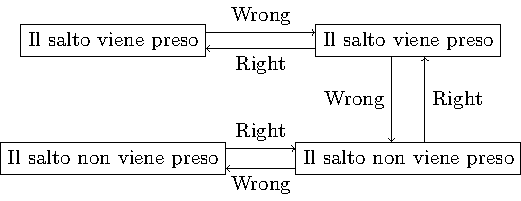
\includegraphics{dynamic_prediction}
    \caption{Esempio predizione dinamica}
    \label{fig:dynamic_prediction}
\end{figure}

Queste predizioni sono salvate in una tabella associativa, dove ad ogni indirizzo di program counter del
salto è associato il valore di relativa predizione.

\subsection{Architetture superscalari}
L'architettura appena vista prende il nome di pipeline lineare, non è più utilizzata perché, come visto, lo speedup teorico è ben diverso dal reale.
Un altro problema dell'architettura è che ogni istruzione attraversa tutti gli stadi, imponendo un periodo di clock coincidente con il tempo dello stadio più lento (uguale alla multiciclo originale).

La soluzione è quindi introdurre non un parziale parallelismo ma un parallelismo totale, sovrapponendo specifiche fasi delle istruzioni.
\\
Nell'architettura che utilizzeremo come riferimento, solo la fase di execute è in parallelo:

\begin{figure}[h]
    \begin{minipage}{.5\textwidth}
        \centering
        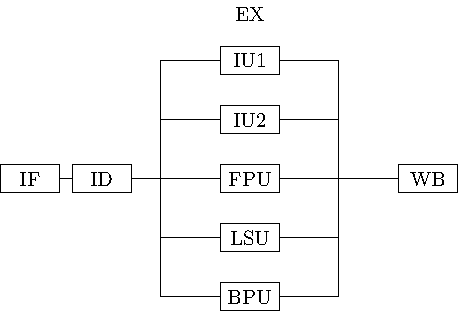
\includegraphics[width=.8\textwidth]{cpu_parallelism}
    \end{minipage}
    \begin{minipage}{.45\textwidth}
        \begin{itemize}
            \item IU1= ALU, per aritmetica intera (1 cck)
            \item IU2=ALU, per aritmetica intera, ma operazioni più complesse come moltiplicazione e divisione (2cck)
            \item FPU=ALU, per virgola mobile (4cck)
            \item BPU \textit{Branch Prediction Unit}
            \item LSU \textit{Load Store Unit}
        \end{itemize}
    \end{minipage}
    \caption{Architettura parallelismo di riferimento}
\end{figure}

Ipotizzando che allo stadio ID (\textit{Instruction Decode}) sia emessa una sola istruzione alla volta, appena messa in esecuzione è eseguita in parallelo con le altre fasi di execute già in esecuzione.

\subsubsection{Problemi dell'architettura}
\begin{enumerate}
    \item \label{prob_1} Date due istruzioni $i$ e $j$, se con $i$ che precede $j$, se $i$ impiega più cicli di clock di $j$ ad essere eseguita,
        l'ordine di completamento può risultare invertito.
    \item \label{prob_2} Può accadere che due istruzioni richiedano nello stesso istante di passare alla fase di writeback, generando un conflitto di risorse.
\end{enumerate}

Per risolvere il problema \ref{prob_1} esistono tre metodi:
\begin{enumerate}
    \item il completamento in ordine (reservation shift register), dove le istruzioni attendono per essere completate secondo l'ordine prestabilito;
    \item il buffer di riordinamento, dove le istruzioni una volta completate scrivono il
loro output su un buffer in cui vengono successivamente riordinate;
    \item attraverso l'history buffer, dove lo stato
coerente può essere ripristinato in presenza di conflitti.
\end{enumerate}

\subsubsection{RSR - Reservation Shift register}
Il primo metodo, meno efficiente, è realizzabile attraverso un RSR (\textit{Reservation Shift Register}).
La scrittura sul registro è effettuata tramite prenotazione.

L'RSR è una tabella di colonne:
\begin{itemize}
    \item \code{V}: bit di validità che indica se la posizione corrente contiene informazioni,
    \item \code{PC}: il program counter dell'istruzione, necessario per il ripristinare uno stato coerente in caso di
        predizione di salto errata
    \item \code{UF}: (\textit{Unità Funzionale}) componente che sta eseguendo l'istruzione
    \item \code{Rd}: Registro destinazione del risultato
\end{itemize}
% Tabella esecuzione
Il riordinamento richiede diversi cicli di clock, e non risolve il problema \ref{prob_2} nel caso di multiple richieste d'accesso alla memoria,
in quanto posso avere una scrittura seguita da una lettura e riscontrare un alea di dato.

Per risolvere questo problema o non si emettono comandi di memorizzazione prima che le istruzioni emesse precedentemente
siano completate, o si considera la memoria come un'unità funzionale quindi store occupa una posizione in RSR in modo
che questa raggiunga la cima quando tutte le istruzioni precedenti sono completate.

\subsubsection{ROB - Reordering Buffer}
Il ROB (\textit{ReOrdering Buffer}) non è in grado di risolvere i problemi d'accesso al buffer, per questo viene utilizzato insieme ad RSR con meno campi.

Nell RSR sono presenti le colonne: \code{V}, \code{UF} ed è aggiunto \code{pROB}, un puntatore alla riga della tabella ROB in è inserita l'unità funzionale.

Nella tabella ROB, sono presenti le colonne:
\begin{itemize}
    \item \code{PC}: Program counter dell'istruzione
    \item \code{Rd}: Registro destinazione
    \item \code{C}: bit di completamento, messo ad 1 quando l'istruzione è completata
    \item \code{RIS}: Risultato dell'istruzione
\end{itemize}

È gestito come un buffer circolare. Il writeback viene eseguito quando l'elemento puntato dalla testa del buffer
circolare è segnato come completato.

\subsubsection{HB - History Buffer}
L' History Buffer è una vera e propria history di tutte le scritture sul register file.
È la soluzione più flessibile delle tre, in quanto permette il completamento fuori ordine delle istruzioni. La cronologia delle scritture garantisce il ripristino di uno stato coerente nel caso di previsione di salto errata.

È gestito come il ROB, un buffer circolare di cui ogni riga contiene i valori:
\begin{itemize}
    \item \code{C}: Flag di istruzione completata
    \item \code{PC}: Program counter dell'istruzione
    \item \code{Rd}: Registro destinazione
    \item \code{OLD}: Valore contenuto nel registro destinazione prima di effettuare il writeback
\end{itemize}

Se ad ogni riga si aggiunge l'informazione \code{EPR} (\textit{Errata Previsione}), quando un'istruzione di salto arriva alla testa dell'HB, se \code{EPR = 1}, blocco l'immissione di nuovi valori, attendendo che le operazioni attive vengano completate (svuotamento della pipeline), ed eseguo il rollback fino a raggiungere la prima istruzione sul percorso sbagliato.


\subsubsection{Considerazioni}
Per l'architettura superscalare, abbiamo presupposto l'emissione ed il ritiro di un'unica istruzione alla volta dalla coda di esecuzione.
Se viene emessa un'unica istruzione alla volta non può mai accadere che viene eseguita più di un'istruzione per ciclo di clock.

Per avere una completa architettura superscalare è necessario ritirare, decodificare ed emettere più istruzioni in parallelo.

\end{document}
